\chapter{Problem Analysis}\label{ch:PA}
The chapter will look into how autonomy has been implemented into vehicles in the real world as well as the safety measures that has to be taken into account for such a vehicle to drive around. Also the ethics behind autonomous vehicles will be discussed followed by an evaluation of different sensors that can be used for such vehicles.

\section{Existing Technologies} \label{Existing technologies}
Self driving cars are a completely new technology that is yet to be commercialised. Although companies, that are creating these automobiles, are yet to sell a single unit, the market is highly competitive in regards to development. 
This section presents different levels of automation and what companies on the market are doing. Since the market is very new, companies will often not provide the information on prices of the cars, what hardware and sensors they use or how they actually control the car, which makes for a difficult gathering of information.


\subsection{Levels of Autonomous Cars}
When discussing self-driving cars it is important to note, that there are varying degrees of autonomy. When comparing the different solutions that currently exist the level of autonomy differs and should be taking into account. 
\begin{enumerate}
\item The first level is concerning driver assistance. Such features are already included in cars today. This could be cruise control, where the car drives with the a constant speed based on commands from the driver behind the wheel. It could also be assisting in acceleration and steering.
\item The second level is partial automation. This is achieved when two or more automated features work simultaneously. An example could be cruise control with automatic breaking. The Tesla Autopilot is a level two autonomous system.
\item Level three heightens the autonomy by having the car being able to drive on its own, especially when driving on the highway. However, the driver is still required to be in the car and being able to take over. This is called conditional automation.
\item For level four, high automation, the car can drive itself without the need for a driver in the car. The car can simply be accessed remotely if necessary. The Waymo car is currently testing for level four autonomy.
\item Level five is full automation. This is car that can drive itself in any conditions. This level of autonomy will be reached in the future \cite{Autonomylevel}\cite{AutonomyLevel2}.
\end{enumerate}


\subsubsection{AGVs and SDVs}
A further distinction to autonomous cars can be made. Automated Guided Vehicles (AGVs) and Self-Driving Vehicles (SDVs) are fundamentally different even though both are autonomous. An AGV is reprogrammed to run on a predetermined route which is controlled by GPS, beacons, magnetic tape etc.. These devices will use sensors and laser to do emergency stop. The SDVs use no driver input and are using sensors, lasers and cameras to control all aspects of steering. This creates a more solid system that can respond to changes in the environment. \cite{otto_motors}



\subsection{Starship Technologies}
Starship Technologies is a London-based company launched by two Skype-cofounders, Ahti Heinla and Janus Friis. They have made an AGV with the purpose of driving around in cities and deliver food or groceries. They move with a maximum speed of 6.5 kph and can avoid obstacles, such as moving humans, detect traffic lights, intersections and crossroads. They operate within a 5 kilometre radius with their nine cameras and GPS. All robots are being supervised from a central location, where they have the possibility to interfere if the vehicle is stuck, crashed or is being stolen. This puts the robot on a level four autonomy. With the appertaining app the user can put down a marker where they want either their food or groceries delivered and the robot will drive up to the building waiting to be unlocked by the user with the app.\\
The robot has already been tested in 100 cities in 20 different countries and have driven collectively more than 150000 kilometres. They have been implemented in Washington DC, London and Hamburg, and the plan is to implement them at campuses in Europe and USA \cite{Starship}\cite{Starship2}.
\begin{figure}[H]
 \centering
  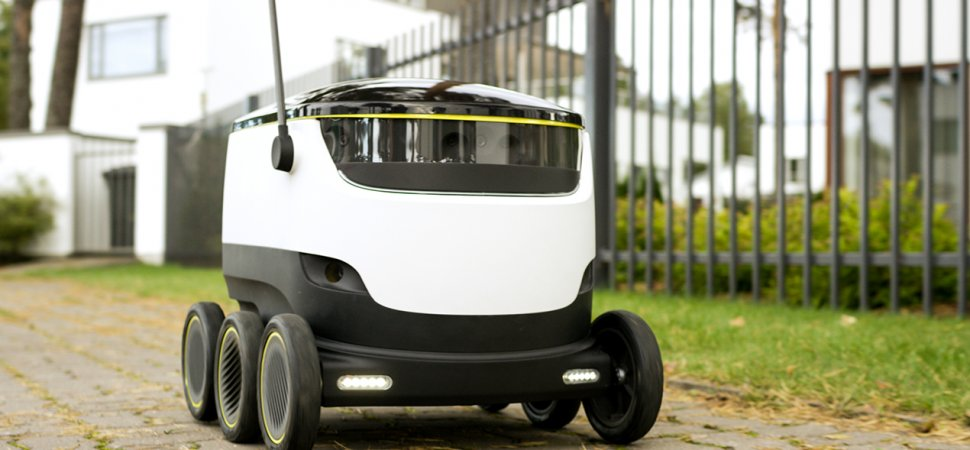
\includegraphics[width=\textwidth]{Figures/ConAnalysis/Market/Starship_robot.jpg}
  \caption{The robot from Starship Technologies\cite{StarshipPic}}
  \label{fig:Starship}
\end{figure}

\subsection{Tesla}
As opposed to the Starship Technologies vehicle, the company Tesla works with SDVs, where a driver behind the wheel is intended. With an update sent to the Tesla Model S in October 2015, they upgraded from just having autopilot and made it possible for the car to drive it self without the need for the driver to control the steering wheel. This is mostly meant for travelling on the highway\cite{Tesla}.
Tesla is yet to go from autonomy level three to four. The cars have the hardware needed in order to drive autonomously, however, the software is not installed on the vehicle as well as there being a safety issue. According the owner of Tesla, Elon Musk, Tesla will achieve the goal of level 5 autonomy in 2020\cite{Tesla2}. %https://www.designnews.com/electronics-test/tesla-will-have-full-autonomy-2020-elon-musk-says/209980870160321
Tesla is unlike other companies very open about which sensor type they use. 
\begin{figure}[H]
\centering
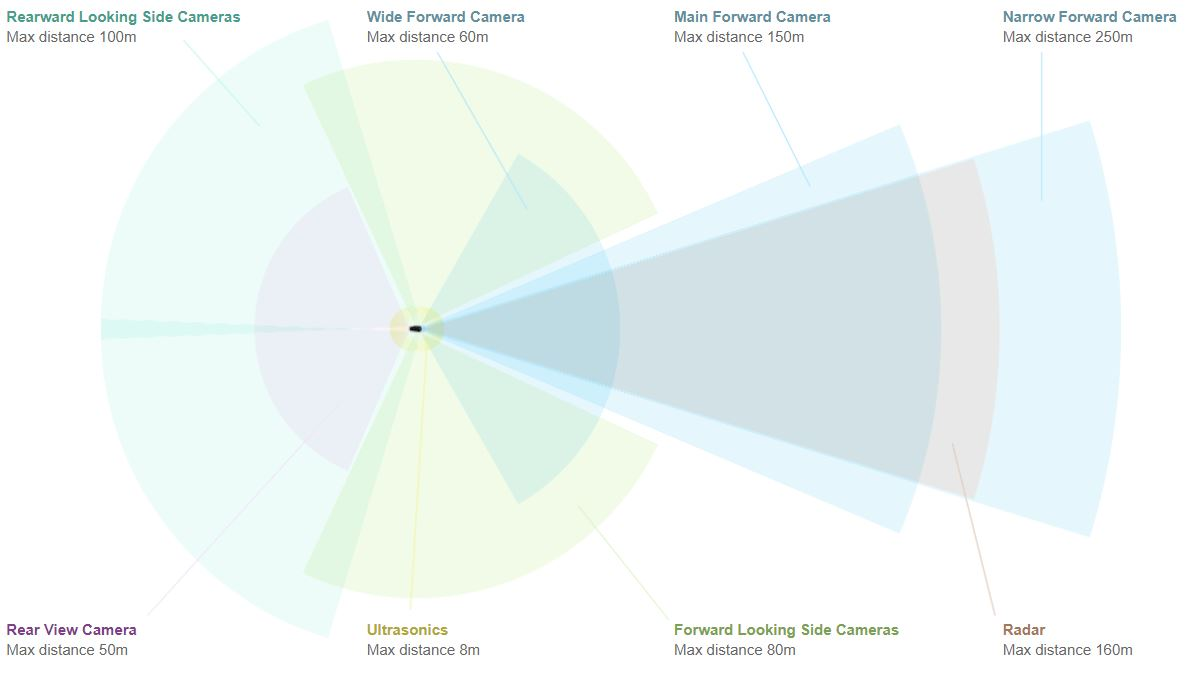
\includegraphics[width=\textwidth]{Figures/ConAnalysis/Market/Tesla.JPG}
\caption{The coverage around a Tesla model provided with distances in meter}
\label{fig:Tesla_market}
\end{figure}
Any Tesla model is equipped with
\begin{itemize}
    \item Eight surround cameras
    \item Twelve ultrasonic sensors
    \item Radar
\end{itemize}
\noindent In figure \ref{fig:Tesla_market} above is an illustration of the ranges and direction of the sensors fitted to the cars. \cite{tesla_autoP}
With the autopilot upgrade in 2015 for the Tesla vehicles, they have naturally been tested a lot in the real world, surpassing 1 billion miles driven with the autopilot. Because this is implemented in the real world it has gathered information in almost any type of environment, be it snow, rain, traffic, fires etc.\cite{Tesla2}\cite{Tesla3}.
%https://cleantechnica.com/2018/11/28/tesla-autopilot-hits-1-billion-miles-why-its-leading/
\begin{figure}[H]
\centering
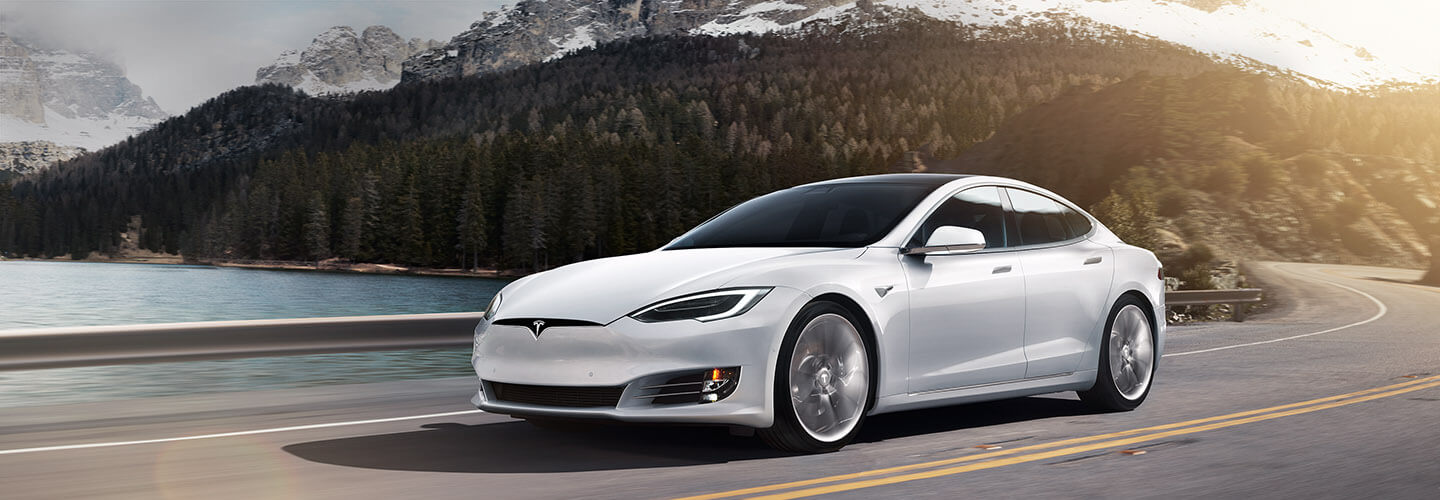
\includegraphics[width=\textwidth]{Figures/ConAnalysis/Market/TeslaMS.jpg}
\caption{The Tesla Model S}
\label{fig:TeslaMS}
\end{figure}
%https://www.tesla.com/da_DK/models


\subsection{Waymo}
Waymo is the former Google Car Project and as Tesla it is a SDV. The car utilises lidar and lasers along with cameras to estimates the velocity and classify the surrounding objects. Waymo is slowly building a fleet of driverless cars, that works as a taxi-service, you can call through a smart phone app, giving the vehicle a level four autonomy.\\ 
The company does not provide a detailed description of sensors and functions that are included with the car. It is, however, possible to get a general idea of this from videos on their website. Here they talk about lidar, lasers, and object classifications. They also provide a small glimpse of the path-planning software as seen in figure \ref{fig:Waymo_Path} bellow \cite{waymo}.
\begin{figure}[H]
\centering
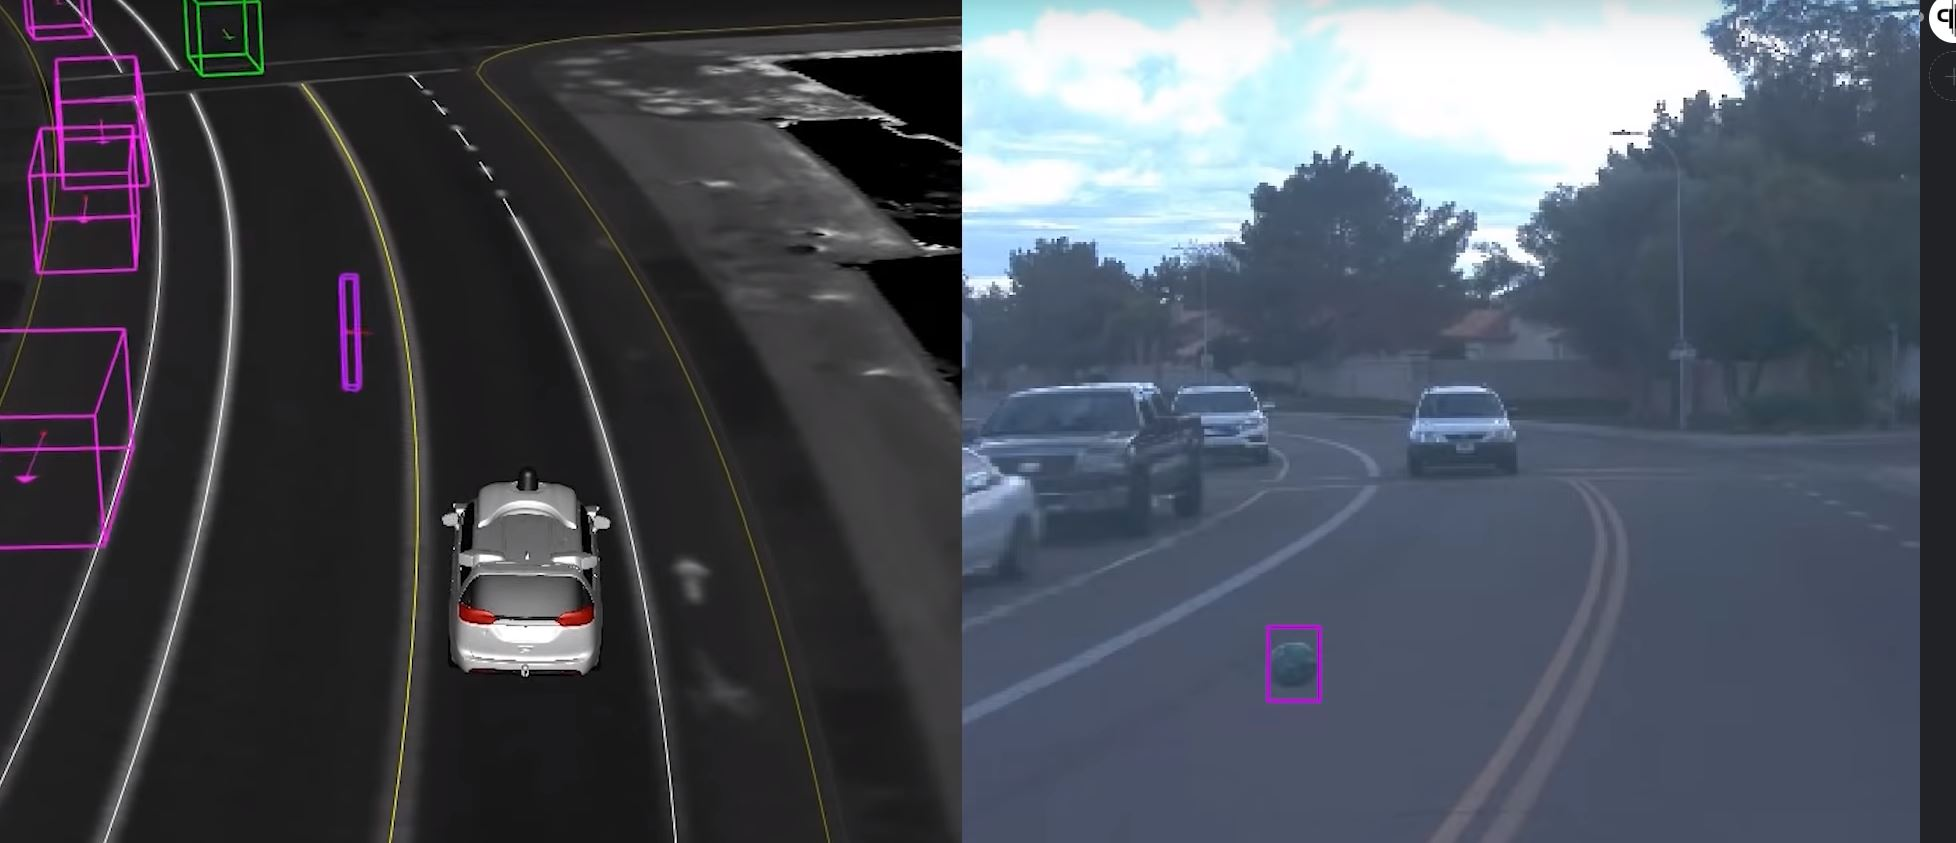
\includegraphics[width=\textwidth]{Figures/ConAnalysis/Market/Waymo.JPG}
\caption{Waymo Path-planning software and image recognition}
\label{fig:Waymo_Path}
\end{figure}

\begin{figure}[H]
\centering
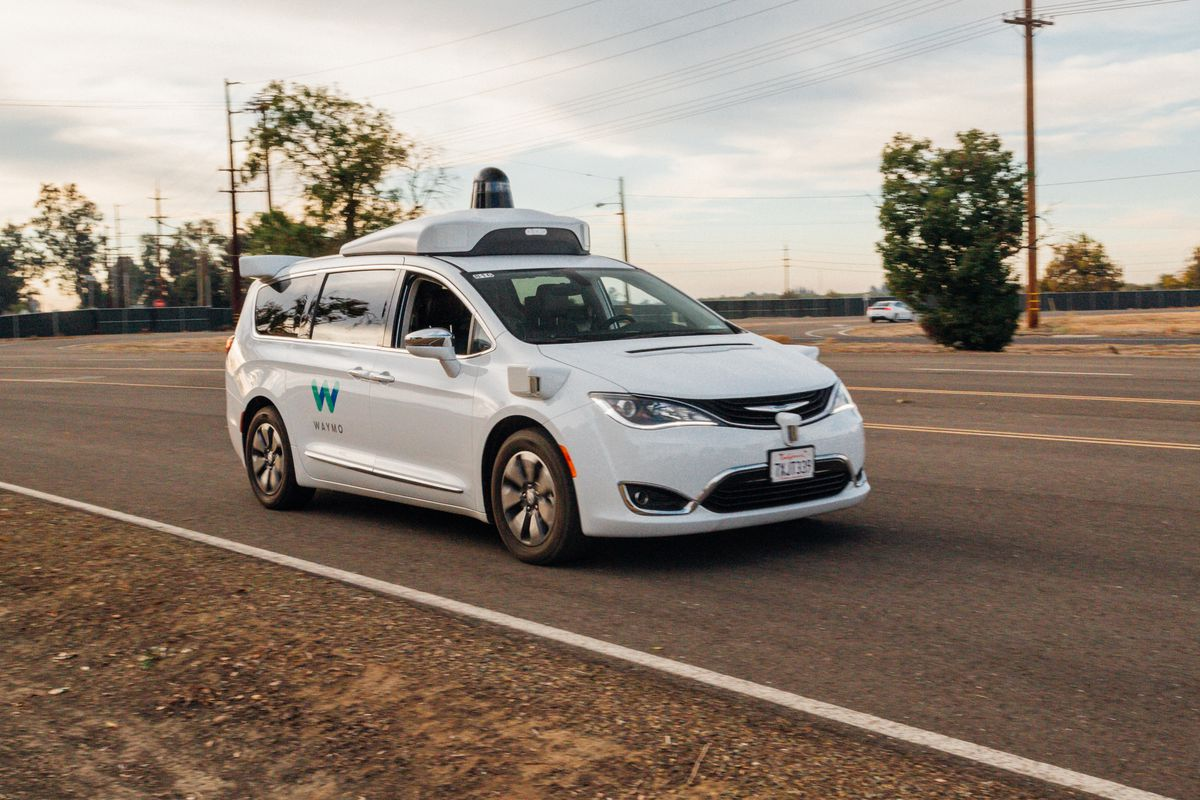
\includegraphics[width=\textwidth]{Figures/ConAnalysis/Market/Waymo.jpg}
\caption{The Waymo vehicle}
\label{fig:Waymo}
\end{figure}
%https://www.theverge.com/2018/10/30/18044670/waymo-fully-driverless-car-permit-california-dmv
\noindent Since the car began being tested in the real world in 2017 it has driven 7 million miles of test on public roads and 10 billion miles in simulation. As of October 2018 the company has been green lit to test their fully driverless cars in California, where it can be tested in the city and on the highway. According to Waymo the car is capable of handling light rain and fog. %Same source as for the picture of the car itself
As opposed to Elon Musk, the CEO of Waymo, John Krafcik does not believe that a fully autonomous level five car that can drive in any condition on any road, will ever going to exist, due to the sensor's limitations in snow and rain, which might never change. %http://macdailynews.com/2019/01/07/waymo-ceo-level-5-fully-autonomous-vehicles-%E2%80%8Awill-never-exist/

%\subsection{Uber}
